\chapter{The Grid and the LCG}

\section{Introduction}
The computing requirements for the LHC are unprecedented. By 2010 CMS alone will require over 60\,PB of storage and 100\,MSI2000~\cite{citeulike:847987} of processing power~\cite{CMS_TDR_PHYS_vol1}. At LHC inception no single computing centre was capable of providing these levels of resources. A mechanism for grouping the resources of multiple centres was required. The grid paradigm popularised by Ian Foster and Carl Kesselman~\cite{citeulike:340626} described such an architecture.

The grid was designed to provide an advanced computing infrastructure suitable for collaborative problem solving within science and engineering. Resources, both computational and storage, were shared amongst collaborating institutions within a dynamic Virtual Organisation (VO). The VO comprises individuals based at different institutions around the world all working towards a common goal. The ultimate aim of grid computing was to provide ubiquitous access to resources such that the user did not need to know where their work was carried out. They simply interacted with the grid and resources were provided. The grid was named by analogy with the power grid: users should consume computing power much as they consume electricity, without knowing the details of how or where it was generated.~\footnote{The concept of computing evolving into such a utility was first popularised by Martin Greenberger in 1964~\cite{citeulike:833641}.}

\section{The LCG}
By the year 2000 no appropriate large scale computational grid existed and so work on a custom-designed solution was started. This resulted in the European DataGrid (EDG)~\cite{citeulike:899441} project which was later succeeded by the Enabling Grids for E-sciencE (EGEE) project~\cite{citeulike:899447}. The LHC Computing Grid (LCG)~\cite{LCG_TDR} was originally based upon the EDG and later the EGEE  implementations plus components from VDT~\cite{vdt}, iVDGL~\cite{iVDGL}, Griphyn~\cite{griphyn} and Datatag~\cite{datatag}~\footnote{Other grid implementations existed i.e. Open Science Grid (OSG) in the USA and NorduGrid in Scandinavia and were used by the LHC experiments. Now they are part of the WLCG (Worldwide LCG).}. This chapter describes the EDG and LCG projects as they were in 2004--2005 when the work described in chapters 5 and 6 was carried out.

\begin{figure}[tb]
  \centering
  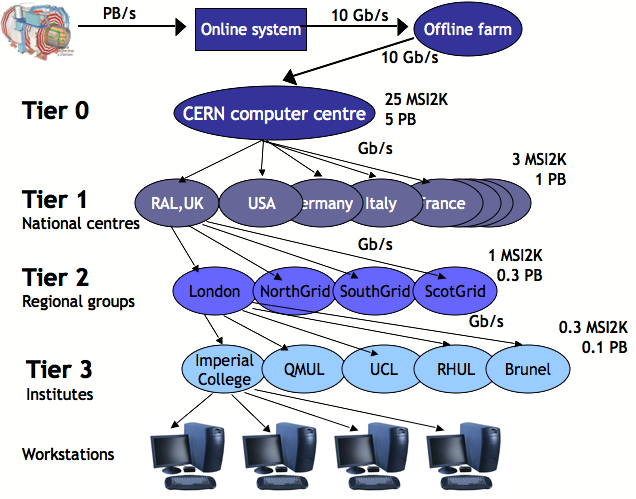
\includegraphics[width=0.9\textwidth]{grid/monarc}
  \caption{The MONARC tiered hierarchy. Network bandwidths are shown for inter-tier links as are computational and storage (disk only) resources for each site in a given Tier. From~\cite{citeulike:421138}.
  \label{fig:monarc}}
\end{figure}

Within the LCG institutions were grouped into a hierarchy derived from the scheme devised by the Models of Networked Analysis at Regional Centres for LHC Experiments (MONARC) project~\cite{Aderholz:2000nk}. This hierarchy took the form of a pyramid (illustrated in Figure~\ref{fig:monarc}) with CERN at the top level (Tier-0). The second level comprised large national computing centres (Tier-1's) followed by regional centres (Tier-2's) and smaller institutes (Tier-3). At each level the resources at a given site decreased, but the number of such sites increased to compensate, from 1 Tier-0 to $\sim$10 Tier-1's, $\sim$50 Tier-2's and an even larger number of Tier-3's.

\begin{figure}[tb]
  \centering
  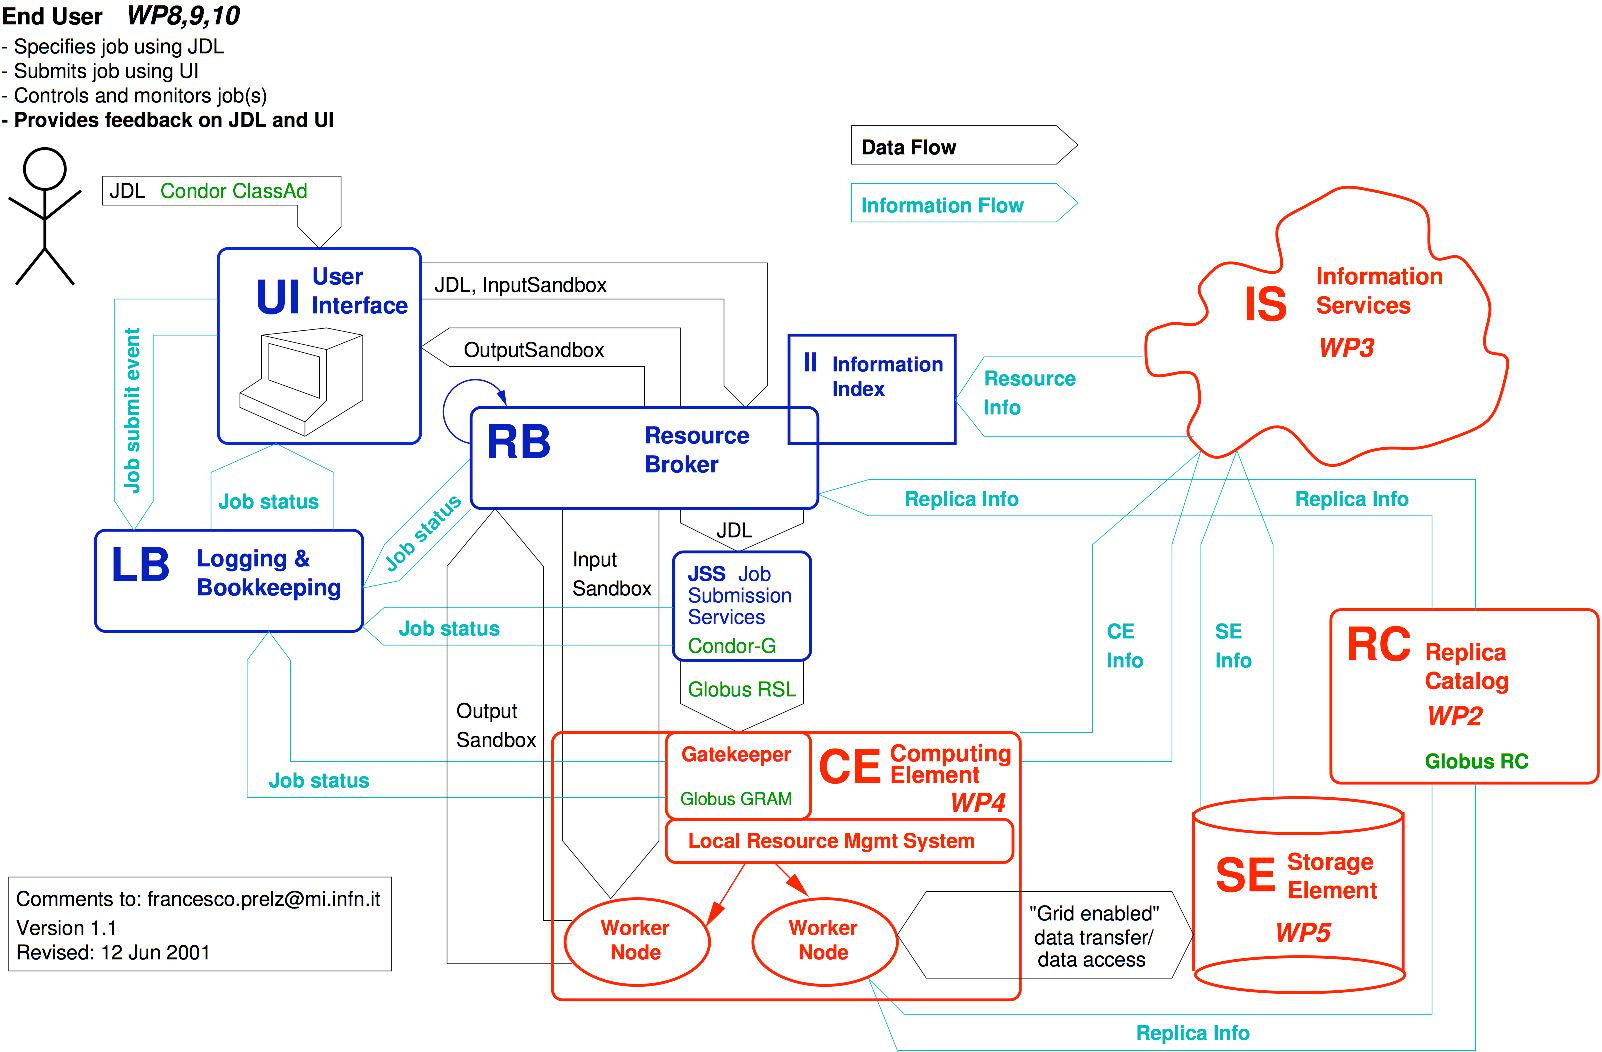
\includegraphics[width=1\textwidth]{grid/LCG-architecture}
  \caption{An overview of the major LCG components. From ~\cite{citeulike:833648}
  \label{fig:LCG-architecture}}
\end{figure}

To provide interaction between users and components a complex software (middleware) architecture was required, as can be seen in Figure~\ref{fig:LCG-architecture}. The User Interface (UI) was the gateway to the grid for users. The installed software allowed the user to manage data and submit computational jobs. 

Data was stored on a site's Storage Element (SE) and recorded in a global file catalogue, known as the Replica Location Service (RLS) or Replica Catalogue. By using the client tools a user could copy data to/from and between SEs. Queries on the RLS were used for data discovery and location.

The Workload Management System (WMS) was provided by the Resource Broker (RB). The RB's role was to accept users' jobs and take responsibility for assigning them to a site for processing. The Computing Element (CE) controlled the processing at a site, receiving jobs from the RB and scheduling them for execution on the site's Worker Nodes (WNs). The Logging and Bookkeeping (LB) system recorded changes in job state and was queried by users to determine the state of their jobs.

The Information Services (IS) listed all the RBs, CEs and SEs and was used by each system, and end users,  to discover and obtain information about the other components.

%%%%%
%Data Management (DM) was provided by the Replica Location Service (RLS) with files stored in Storage Elements (SE). The Information Services (IS) listed all the RB's, CE's and SE's and was used by each system to discover and query other components.
%%%%%

\subsection{Data Management}
The LCG data management system was specifically designed to cope with the types of data produced by particle physics experiments: i.e. large amounts of read-only data. It had also been designed to provide high levels of data availability and integrity with multiple distributed file replicas. To facilitate this the RLS provided the concepts of Logical File Name (LFN), the canonical name by which a file was known, and Physical File Name (PFN), a name referring to a specific file instance. A user would refer to a file by its LFN, the RLS would resolve the best replica and this instance was used in the data operation. As well as holding the LFN/PFN mapping the RLS could also contain a limited number, O(10), file metadata fields. It was generally assumed that files within the RLS were read-only so synchronisation between replicas was not supported.

%LCG's policy was to send jobs to data: if a job required a certain file it was sent to a site which held a copy. This was achieved by the user specifying the required LFN with the job and the RB querying the RLS to find the replica PFNs and hence hosting sites. The RB then submitted the job to one of those sites.

\subsection{Workload Management}
To submit a job the user first had to describe their job in a Job Description Language (JDL) file~\cite{citeulike:835506}.  This file was written in the Classified Advertisements (ClassAds)~\cite{citeulike:835507} syntax and listed the job structure and attributes. Fields included information such as executable name and arguments. It was also possible to specify requirements for the job which were used by the RB to determine an appropriate site to run the job. Typical requirements included criteria such as operating system, site capacity and processing time limits. 

In the JDL the user could also specify input and output files. There were two mechanisms for file handling: small files (e.g. log files and text files) were sent with the job whereas large data files were saved to SEs and registered with the RLS. Input (output) files sent with the job were said to be part of the input (output) sandbox. As well as containing the user-defined input files, the input sandbox contained the users executable and an optional file used as standard input for the job. The output sandbox contained the user defined output files and the standard output and error streams from the job.

Once the user had a JDL file they could submit the job via the software on the UI to an RB. The RB received both the job and the input sandbox then selected the most appropriate CE taking into account the specified requirements, a process known as match-making. Once a CE received the job it was added to the local batch queue and scheduled for execution. Before the job started, the WN downloaded the input sandbox from the RB. The user's job was then executed. Once the job had finished the output sandbox was transferred to the RB. Changes in job state were recorded to the LB. This information was then available to the user. The output sandbox was retrievable from the UI.

The WMS interacted with the RLS when the user specified one or more LFNs in the JDL. It was LCG policy to send jobs only to sites which hosted all of the required data. Thus, if a user specified any input LFNs, the RB contacted the RLS, retrieved the list of hosting sites and only considered those in the match-making decision. At the end of the job it could copy any output files to an SE and register them with a user-provided LFN.

%A job could interact with both input and output files. The job could interact with the RLS if the user specified an LFN. It was LCG policy for jobs requiring input data to be sent to a site which hosted all the necessary files. This was achieved by the user specifying the input LFN's in the JDL, these were then available to the RB when it received the job. When the RB attempted to match the job requirements to the available sites it would contact the RLS and only consider sites which hosted all the required data. 

%Files that were not registered could be sent with the job to the CE via the RB, this was called the input sandbox. At the end of the job output files could either be saved to an SE and registered with the RLS or sent back to the RB where they could be retrieved by the user on the UI, this was called the output sandbox.

%Once the user had a JDL file they could submit it via the software on the UI to an RB. The RB received both the job and the input sandbox then selected the most appropriate CE and sent the job to it. Once a CE received a job it was added to the local batch queue and scheduled for execution. Once the job finished the output was handled and the job was sent back to the RB along with the output sandbox. The user could retrieve the contents of the output sandbox, and query the status of their jobs, by using the software on the UI.

\subsection{LCG object persistency}
As well as core grid functionality the LCG project developed related software services for the LHC experiments. One of these was POOL (Pool Of persistent Objects for LHC)~\cite{citeulike:899448} which provided object persistency and file input/output (IO). This system was used by 3 of the LHC experiments, including CMS, in their event data model.

POOL used the LFN/PFN convention and required a file catalogue to store these. This catalogue was used to locate files when users referred to them with an LFN. Multiple file catalogue implementations existed including the RLS, MySQL~\cite{citeulike:835488} databases and XML files. The user had to provide a contact string for a POOL file catalogue before requesting any file operations. POOL provided an Application Programming Interface (API) for queries of the file catalogue. This API allowed queries of LFNs, PFNs and metadata as compared to the native RLS API that was restricted to queries of LFN-PFN only.

When an application used POOL for writing to a file it was automatically added to the file catalogue. When a file was accessed the application/user used the LFN and POOL would consult the catalogue to locate a physical replica to use.

% When saved files were added to the catalogue and they had to be listed before they could be accessed. The POOL file catalogue component consisted of an API and backend technology. The possible backends included the RLS, MySQL and XML files. The same information as in the RLS could be stored in any of these. 

%The POOL file catalogue API allowed queries of LFNs, PFNs and metadata where the native RLS API only allowed LFN/PFN queries. Applications using POOL would use the LFN to specify a file, POOL would use the catalogue to locate a physical replica and use that for all further operations.

This architecture did not make applications grid-aware, however, because files could only be accessed within a site. POOL had no mechanism for resolving the ``best'' PFN or for trying multiple replicas. If a PFN referring to a file hosted elsewhere was returned it would cause the application to fail.

\section{Summary}
The LHC computing requirements were greater than any single site could provide. Therefore the LCG was developed to provide a distributed computing infrastructure for the LHC experiments. This infrastructure provided both data and workload management. However these were not seamless and did not provide all of the necessary functionality. If required, more advanced and custom features had to be implemented by each experiment on top of the LCG. The system developed for CMS is described in the next chapter.